\section{Параметрическое представление многомерных каналов связи}

\begin{frame}
	\frametitle{Модель системы связи}
	
	Принимаемый сигнал систем с множеством поднесущих (например, OFDM), приёмных и передающих антенн (MIMO) можно описывать в общем виде как
	\begin{equation}
	\label{eq:1}
	[\ten{Y}]_{(\ti,\fri,\rxi)} = \sum_{\txi=1}^{\Ntx} [\ten{H}(\pars)]_{\ti,\fri,\rxi,\txi} \cdot [\ten{S}]_{\ti,\fri,\txi} + [\ten{N}]_{(\ti,\fri,\rxi)}
	\end{equation}
	
	\begin{description}[longest label]
		\item[$\ten{S}\in\compl^{\Nt\times \Nf \times \Ntx}$] тензор отсчётов передаваемого сигнала
		\item[$\ten{Y}\in\compl^{\Nt\times \Nf \times \Nrx}$] тензор отсчётов принятого сигнала
		\item[$\ten{H}(\pars)\in\compl^{\Nt\times \Nf \times \Nrx \times \Ntx}$] тензор отсчётов принятого сигнала
		\item[$\ten{N}\in\compl^{\Nt\times \Nf \times \Nrx}$] тензор отсчётов аддитивного шума/помехи
		\item[$\pars\in\real^\Npars$] вектор неизвестных (скрытых) параметров канала (например, направления прихода/излучения сигналов, расстояние до источников/отражателей и их относительная скорость и т.д.)
	\end{description}
		
\end{frame}
\note{
	Сигналы и модели каналов в современных коммуникационных системах обладают многомерной структурой. Например, формулируя представление передаваемых сигналов в общем виде, могут быть выделены такие измерения как частота (для систем с множеством поднесущих, таких как OFDM), время и пространство (отдельно для передающих и приёмных антенн).
}

\begin{frame}
	\frametitle{Многолучевая модель канала связи}
	
	\begin{assumption}
		\label{as:1}
		На каждой поднесущей $\fri$ и в каждый момент времени $\ti$, канал связи представляется как суперпозиция узкополосных каналов передачи (лучей) с постоянной частотной передаточной характеристикой.
	\end{assumption}
	
	Тогда:
	\begin{equation}
	\label{eq:3}
	\ten{H}(\pars)=\sum_{\pai\in\Spai} \ten{H}_\pai(\pars)
	\end{equation}
		
	\begin{description}[longest label]
		\item[$\Spai$] множество путей от $\txi$-й антенны
		\item[$\ten{H}_\pai(\pars)$] канал связи $\pai$-го пути от $\txi$-й передающей антенны
	\end{description}

	Тензорные разложения: 
	\begin{itemize}
		\item Сингулярное разложение Высокого порядка (Higher Order Singular Value Decomposition - HOSVD \cite{Haardt08})
		\item Каноническое (Canonical Polyadic Decomposition - CPD \cite{Bros99, Roemer13})
		\item ...
	\end{itemize}
\end{frame}
\note{
	Многолучевая параметрическая модель канала связи подразумевает его описание как суперпозиции конечного числа дискретных путей распространения (лучей). Такой подход создаёт предпосылки к использованию тензорного представления каналов связи с последующим использованием методов тензорных разложений, таких как Сингулярное разложение Высокого Порядка (HOSVD), Каноническое разложение тензора (CPD), и другие.
}

\section{Оценивание параметров широкополосных каналов связи}

\begin{frame}
	\frametitle{{\large Оценивание параметров широкополосных каналов связи I}}
	
	\begin{minipage}[t]{0.47\linewidth}
		{
		\setbeamercolor{block body}{bg=structure!10}
		\setbeamercolor{block title}{bg=structure!20}
		\setbeamertemplate{blocks}[rounded][shadow]
		\begin{block}{}
			\begin{itemize}
				\item OFDM cистема с одной передающей антенной (SIMO)
				\item Отражённый сигнал принимается массивом приёмных антенн со-расположенным с передающей антенной
			\end{itemize}		
		\end{block}
		}
	\end{minipage}
	\hfill
	\begin{minipage}[t]{0.47\linewidth}
		\begin{center} \textbf{Рассматриваемая система}
		\end{center}
		\center{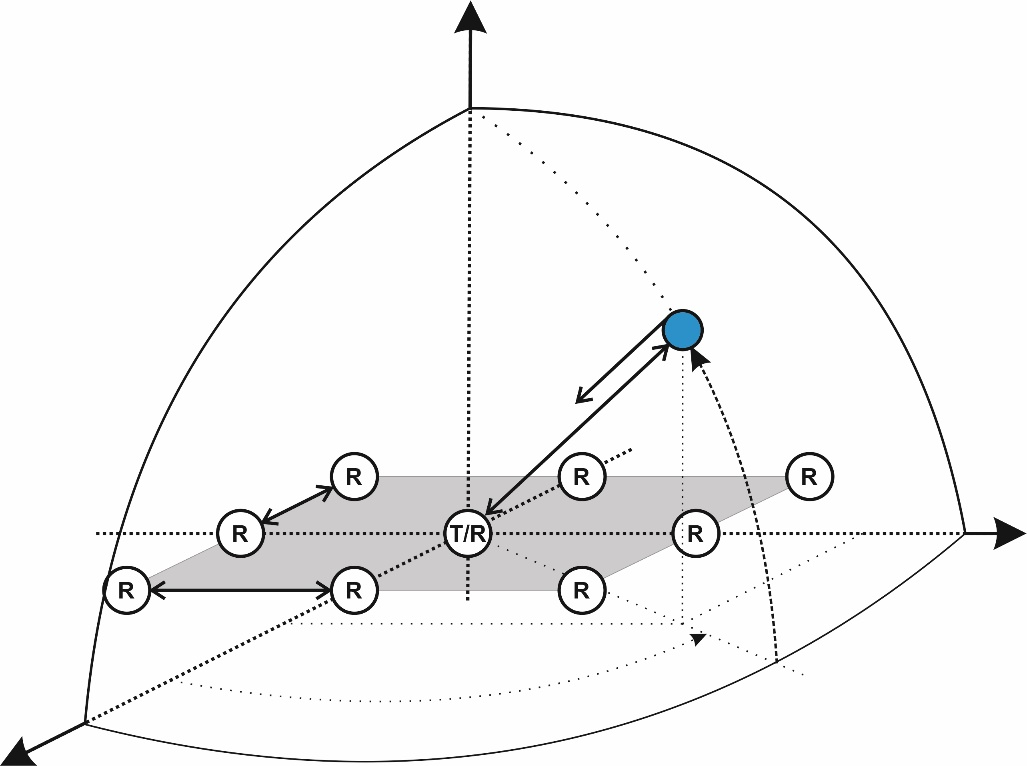
\includegraphics[width=1\linewidth]{rpresentation/atRwEi.jpg}}
	\end{minipage}
	\vfill			
	\begin{equation}
	\begin{aligned}
	\label{eq:5}
	[\ten{H}_\pai(\pars)]_{(\ti,\fri,\rxi_\te{x},\rxi_\te{y})} =\underbrace{\tgaini \cdot e^{-j2\pi \lfr \delay}}_{\gaini} \cdot 
	\underbrace{e^{-j2\pi \scs \fri \delay}}_{b_{\pai,\fri}^f} \cdot \\
	\underbrace{e^{j2\pi \frac{\color{red}\sfr\color{black} \ts\ti}{c} \vrel}}_{b_{\pai,\ti,\fri}^t} \cdot
	\underbrace{e^{-j2\pi \frac{\color{red}\sfr}{c} \delta_{\rxi_\te{x}}^{r,\te{x}}}}_{b_{\pai,\rxi_\te{x},\fri}^\te{x}}
	\underbrace{e^{-j2\pi \frac{\color{red}\sfr}{c} \delta_{\rxi_\te{y}}^{r,\te{y}}}}_{b_{\pai,\rxi_\te{y},\fri}^\te{y}}
	\end{aligned}
	\end{equation}
	\vfill
\end{frame}
\note{
	Рассматрим систему с одной передающей и массивом приёмных антенн. Формула 3 описывает параметризацию одного луча в такой системе. Как выделено в формуле, фазовые сдвиги между отдельными антеннами, равно как и набег фазы в результате Допплеровского сдвига от символа к символу зависят от частоты (выделено красным). В такой постановке параметрическое описание лучей не позволяет напрямую использовать упомянутые тензорные разложения, равно как и множество других методов оценивания, предназначенных для узкополосных систем.
	
	В связи с этим была предложена методика предварительной обработки сигналов, позволяющая уменьшить отклонения модели данных в широкополосной системы от эквивалентой узкополосной.
}

\tikzset{
	myarrow/.style={
		draw,
		fill=blue,
		single arrow,
		minimum height=3.5ex,
		single arrow head extend=1ex
	}
}
\newcommand{\arrowdown}{%
	\tikz [baseline=-1ex]{\node [myarrow,rotate=-90] {};}
}
\begin{frame}
	\frametitle{{\large Оценивание параметров широкополосных каналов связи II}}	
	\centering
	\vfill
	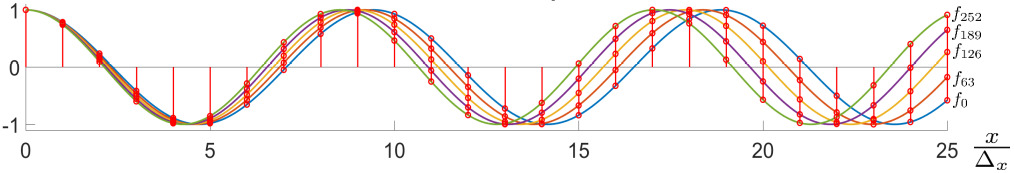
\includegraphics[width=1\linewidth]{rpresentation/wideband} \\
	\vfill
	\arrowdown
	\vfill
	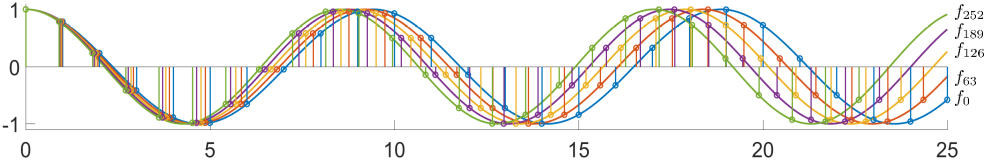
\includegraphics[width=1\linewidth]{rpresentation/iwideband}
	\vfill
	{
		\footnotesize
		\setbeamercolor{block body}{bg=brown!10}
		\setbeamercolor{block title}{bg=brown!20}
		\setbeamertemplate{blocks}[rounded][shadow]
		\begin{block}{Публикации}
			\begin{itemize}
				\item Efficient multidimensional parameter estimation for joint wideband
				radar and communication systems based on OFDM. /. — J. Zhang
				[и др.] //. — New Orleans, LA : IEEE, 2017. — С. 3096—3100.
				\item Efficient Multidimensional Wideband Parameter Estimation for
				OFDM Based Joint Radar and Communication Systems. /. —
				I. Podkurkov [и др.] // IEEE Access. — 2019. — Т. 7. —
				С. 112792—112808. 
			\end{itemize}
		\end{block}
	}
\end{frame}
\note{
	Идея заключается в следующем. Для простоты представим на рисунке изменение фазы вдоль одного измерения антенн прямоугольного массива антенн (как на рисунке на предыдущем слайде). Увеличение f\_i вызывает дополнительный набег фаз для поднесущих с высокой частотой. Однако, если подстраивать период дискретизации (расстояние между антеннами) в зависимости от частоты, можно было бы скоменсировать дополнительный набег фазы и получить данные, эквивалентные узкополосной системе. Так как физически это невозможно, простым решением является использование интерполяции для получения отсчётов с нужным периодом на каждой частоте.
}

\begin{frame}
	\frametitle{{\large Оценивание параметров широкополосных каналов связи III}}
	\begin{minipage}[с]{1.1\linewidth}
		\begin{center} 
			\textbf{Результаты компьютерного моделирования}
			\center{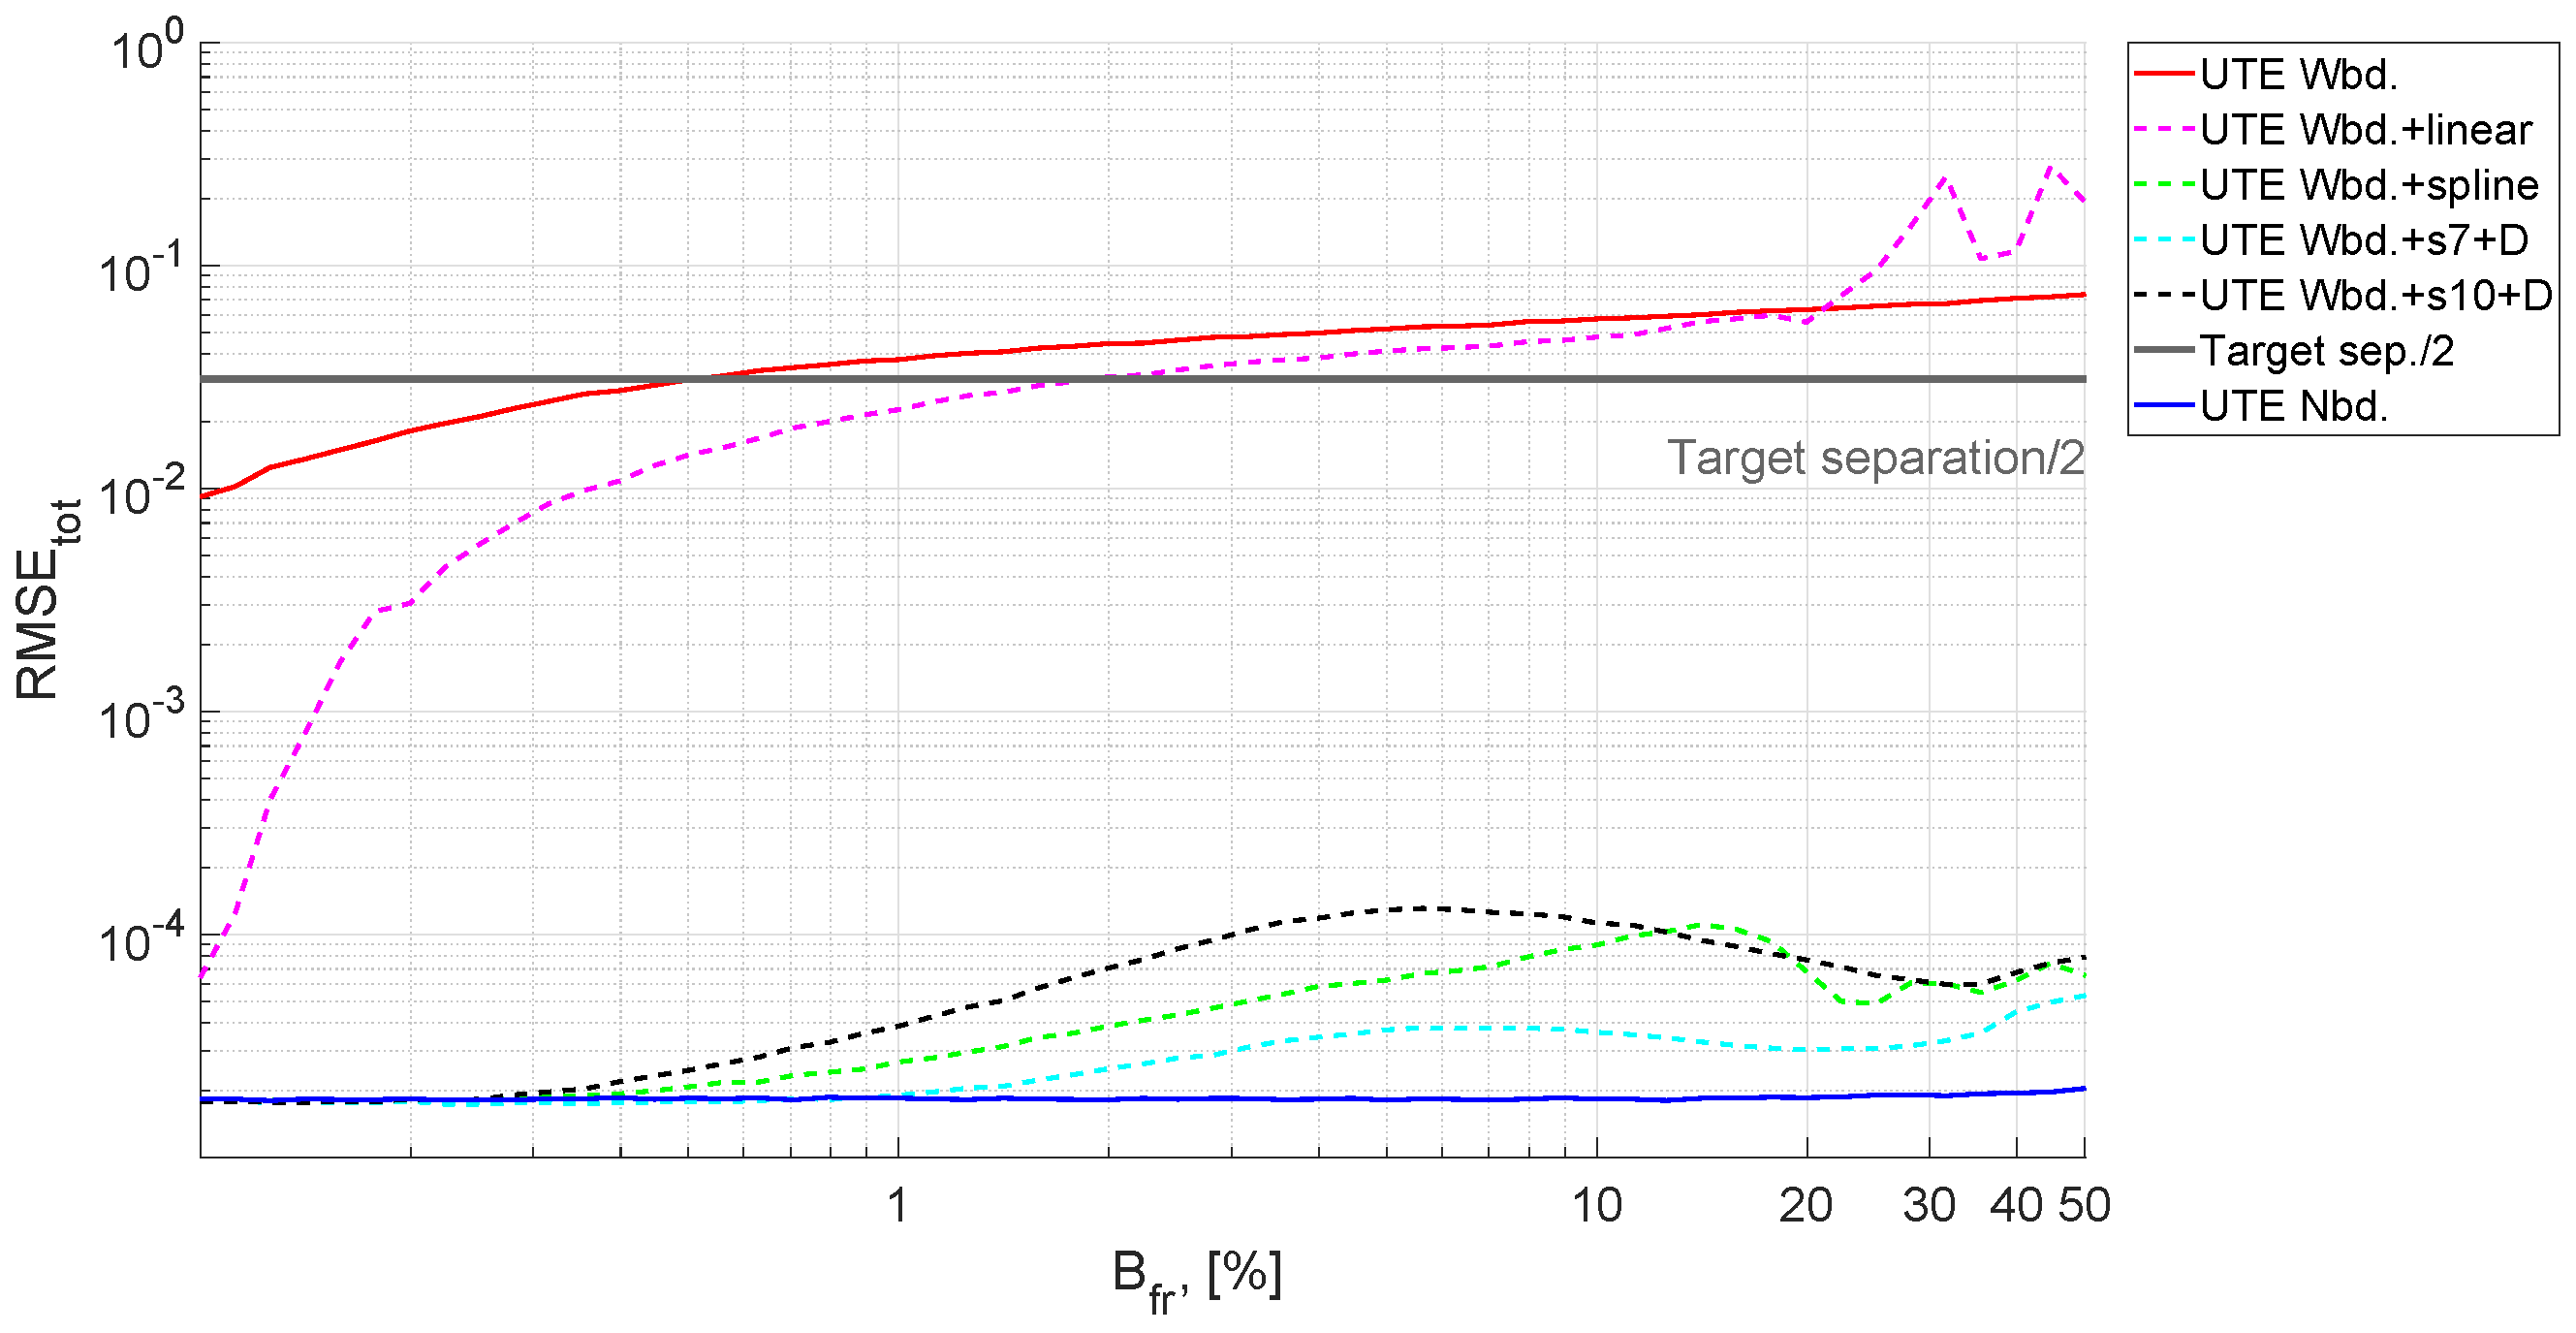
\includegraphics[width=0.8\linewidth]{FRAC_ed_final}}
		\end{center}
	\end{minipage}
	\vfill
	{
		\footnotesize		
		\setbeamercolor{block body}{bg=structure!10}
		\setbeamercolor{block title}{bg=structure!20}
		\setbeamertemplate{blocks}[rounded][shadow]
		\begin{description}
			\item [UTE] Unitary Tensor ESPRIT \cite{Haardt08}
			\item [Wbd./Nbd.] использование широкополосной/узкополосной модели данных
			\item [Linear/spline/s7/s10] интерполяция с помощью сплайнов 1/3/7/10 порядка, соответственно
		\end{description}
	}
\end{frame}
\note{
	Результаты компьютерного моделирования показывают, что применение предварительной обработки с помощью интерполяции данных позволяет существенно увеличить эффективность оценивания в широкополосной системе, в то же время имея возвожность использовать узкополосный алгоритмы оценивания.
}


\section{Оценивание параметров каналов связи в ближнем поле}

\begin{frame}
	\frametitle{{\large Оценивание параметров каналов связи в ближнем поле I}}
	
	\begin{minipage}[t]{0.47\linewidth}
		{
			\setbeamercolor{block body}{bg=structure!10}
			\setbeamercolor{block title}{bg=structure!20}
			\setbeamertemplate{blocks}[rounded][shadow]
			\begin{block}{}
				\begin{itemize}
					\item Рассматривается MIMO Radar система \cite{Singh2017a} \cite{Podkurkov2018}
					\item Используется сферическая модель фронта волны
				\end{itemize}		
			\end{block}
		}
	\end{minipage}
	\hfill
	\begin{minipage}[t]{0.47\linewidth}
		\begin{center} \textbf{Сферический фронт волны}
		\end{center}
		\center{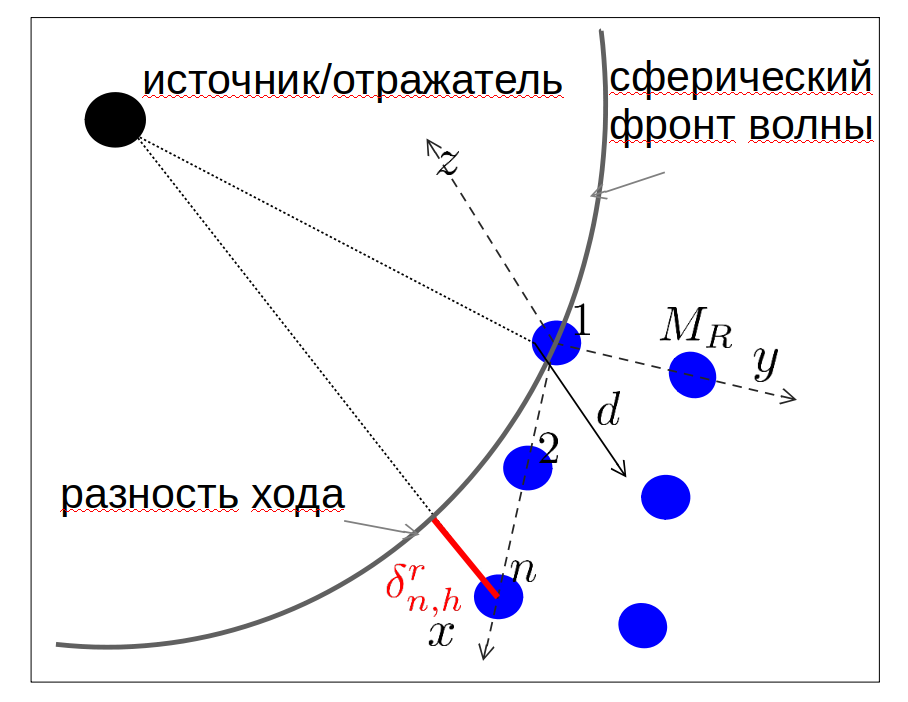
\includegraphics[width=1\linewidth]{rpresentation/nearfield}}
	\end{minipage}
	\vfill			
	\begin{equation}
	\label{eq:6}
	\delta_{\rxi,\pai} = \sqrt{ (x_\pai-x_\rxi)^2 + (y_\pai-y_\rxi)^2 + (z_\pai-z_\rxi)^2} -\rho_\pai\text{\ \ }\forall \rxi,\pai	
	\end{equation}
	\vfill	
	\begin{description}
		\item[$x_\rxi$, $y_\rxi$, $z_\rxi$] Декартовы координаты $\rxi$-й приёмной антенны
		\item[$x_\pai$, $y_\pai$, $z_\pai$] Декартовы координаты $\pai$-го источника/отражателя антенны
		\item[$\rho_\pai$] расстояние до $\pai$-го источника/отражателя антенны
	\end{description}
\end{frame}
\note{
	Тензорные разложения открывают новые возможности для построения алгоритмов оценивания каналов связи. В частности, использование Канонического тензорного разложения в системе с отражателями/источниками в ближнем геометрическом поле позволило разработать новый алгоритм определения углов прихода сигналов и расстояния с использованием сферической модели фронта волны, для которой разности хода фронта между антеннами имеют нелинейную зависимость от положения источника/отражателя.
}

\begin{frame}
	\frametitle{{\large Оценивание параметров каналов связи в ближнем поле II}}
	
	\begin{minipage}[t]{0.3\linewidth}
		{
			\small
			\setbeamercolor{block body}{bg=structure!10}
			\setbeamercolor{block title}{bg=structure!20}
			\setbeamertemplate{blocks}[rounded][shadow]
			\begin{block}{}
				Разработан алгоритм локализации источников \cite{Podkurkov2018}, позволяющий получать несмещённые оценки азимута, угла места и расстояния до источника/отражателя с использованием произвольной геометрии приёмного массива антенн		
			\end{block}
		}
	\end{minipage}
	\hfill
	\begin{minipage}[t]{0.64\linewidth}
		\begin{center}
			\textbf{Результаты компьютерного моделирования}
		\end{center}
		\center{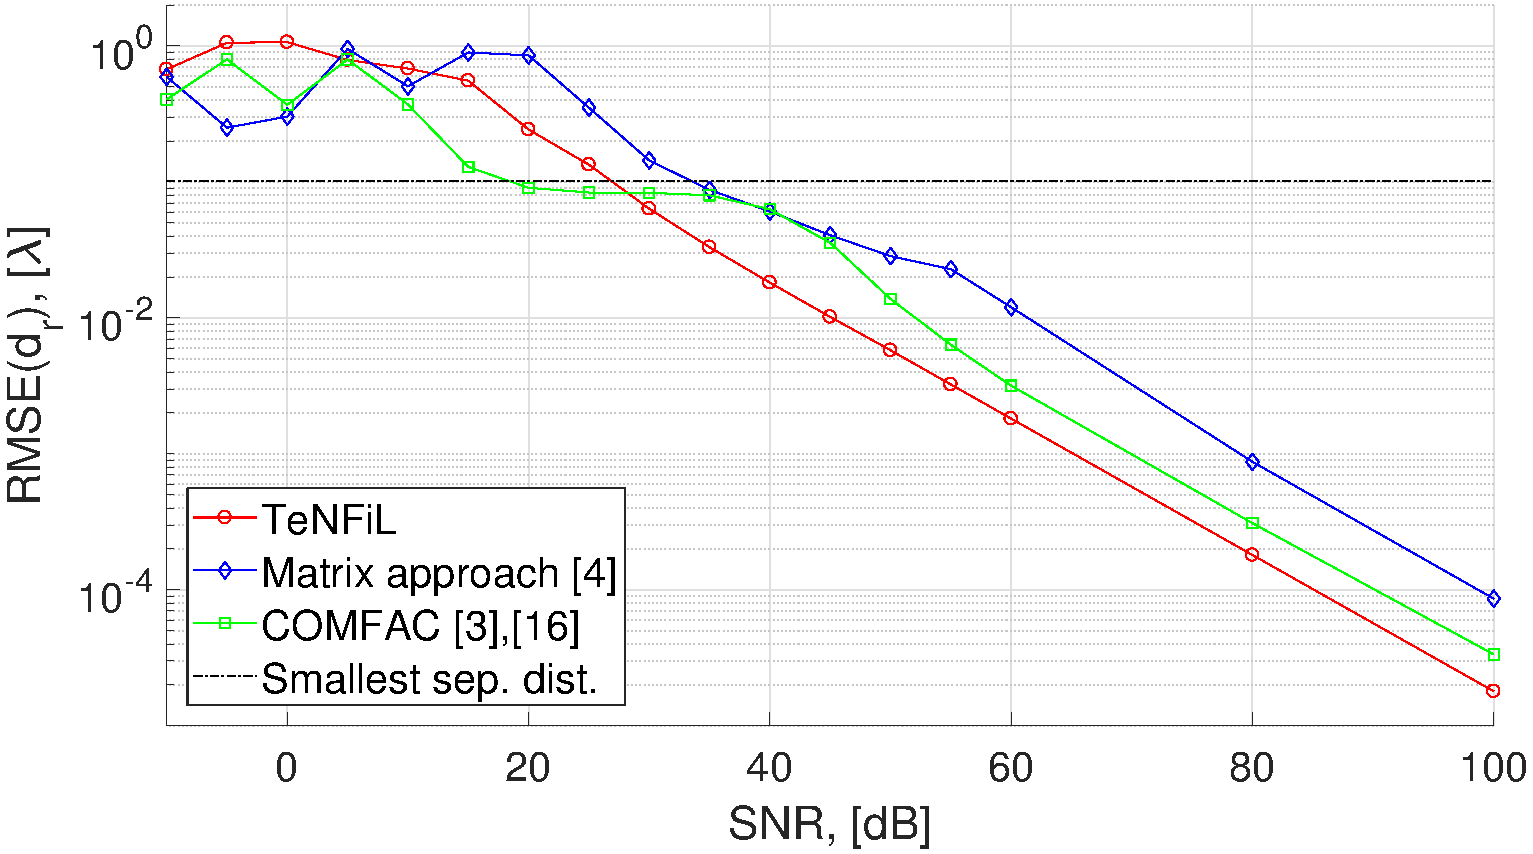
\includegraphics[width=1\linewidth]{mse_dt_onenan}}
		\vfill
		\begin{description}
			\item[TeNFiL] - разработанный метод оценивания
		\end{description}
	\end{minipage}
	\vfill
	{
		\footnotesize
		\setbeamercolor{block body}{bg=brown!10}
		\setbeamercolor{block title}{bg=brown!20}
		\setbeamertemplate{blocks}[rounded][shadow]
		\begin{block}{Публикации}
			\begin{itemize}
				\item Tensor-Based Near-Field Localization in Bistatic MIMO Radar
				Systems. /. — I. Podkurkov [и др.] //. — Bochum, Germany :
				VDE, 2018. — С. 1—8.
			\end{itemize}
		\end{block}
	}
\end{frame}
\note{
	Каноническое разложение позволило получить точные фазовые сигнатуры источников на приёмном массиве антенн, дающие возможность получить несмещённые оценки положения (углов прихода и расстояния). На графике изображено сравнение с аналогичными алгоритмами, TeNFiL - предложенный метод.
}

\section{Анализ потенциальных характеристик оценивания параметров каналов связи.}

\begin{frame}
	\frametitle{Анализ потенциальных характеристик оценивания параметров каналов связи I}
	{
		\setbeamercolor{block body}{bg=structure!10}
		\setbeamercolor{block title}{bg=structure!20}
		\setbeamertemplate{blocks}[rounded][shadow]
		\begin{block}{}
			\begin{itemize}
				\item Аддитивная помеха имеет распределение в виде произвольной смеси Гауссовских распределений
				\item Анализ проводится с помощью вычисления границы Крамера-Рао
			\end{itemize}		
		\end{block}
	}
	{
	\setbeamercolor{block body}{bg=structure!10}
	\setbeamercolor{block title}{bg=structure!20}
	\setbeamertemplate{blocks}[rounded][shadow]
	\begin{block}{Метод вычисления границы Крамера-Рао}
		\begin{itemize}
			\item Аппроксимация промежуточной ("шумовой") матрицы Фишера с помощью метода Монте-Карло
		\end{itemize}	
	\end{block}
	}
	{
		\footnotesize
		\setbeamercolor{block body}{bg=brown!10}
		\setbeamercolor{block title}{bg=brown!20}
		\setbeamertemplate{blocks}[rounded][shadow]
		\begin{block}{Публикации}
			\begin{itemize}
				\item Подкурков, И. А. — Потенциальные характеристики оценивания
				направлений прихода сигналов в условиях негауссовских
				помех. /. — И. А. Подкурков, А. Ф. Надеев // Вестник
				Марийского государственного технического университета.
				Серия: Радиотехнические и инфокоммуникационные
				системы. — 2019. — Т. 1, No 4. — С. 16—26.
			\end{itemize}
		\end{block}
	}		
\end{frame}
\note{
	Анализ потенциальных характеристик осуществлялся с помощью численной аппроксимации границы Крамера-Рао, полученной с помощью метода Монте-Карло. При этом сначала аппроксимируется промежуточная матрица Фишера задачи, в которой неизвестными параметрами считаются отсчёты шума/помехи. Далее, вычисление матрицы Фишера относительно неизвестных параметров осуществляеются с помощью преобразования смены переменных и инверсии полученной матрицы.
	
	Стоит отметить, что вычисление границы Крамера-Рао для произвольного распределения помехи является крайне сложной задачей, в частности для смесевых распределений и в литературе встречается лишь для частных случаев.
}

\begin{frame}
	\frametitle{Анализ потенциальных характеристик оценивания параметров каналов связи II}
	\begin{minipage}[t]{0.47\linewidth}
		\begin{center}
			\textbf{Результаты компьютерного моделирования}
		\end{center}
		\center{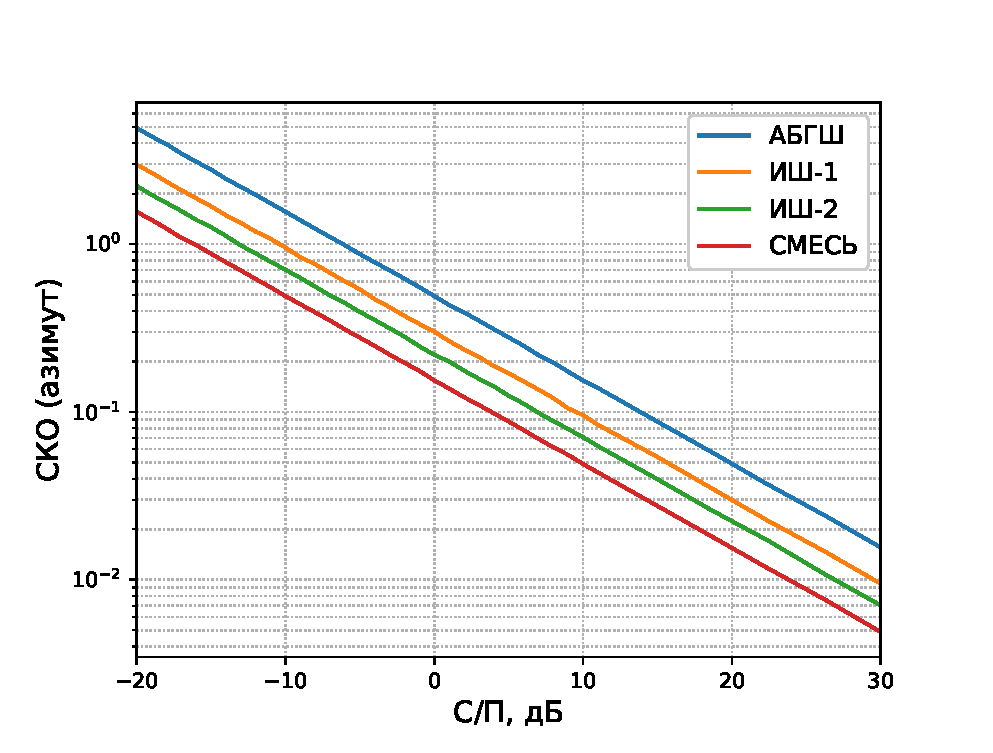
\includegraphics[width=1.3\linewidth]{Fig_2}}
	\end{minipage}
	\hfill
	\begin{minipage}[t]{0.47\linewidth}
		{
			\scriptsize
			\begin{description}
				\item [АБГШ] Аддитивный Белый Гауссовский шум
				\item [ИШ-1] аддитивная помеха задана циклично-симметричной смесью двух компонент с различными дисперсиями ("импульсный шум")
				\item [ИШ-2] аддитивная помеха задана смесью двух компонент с различными дисперсиями и корреляцией между квадратурными компонентами шума
				\item [СМЕСЬ] произвольная смесь компонент с ненулевыми средними и одинаковыми кофариацонными матрицами
			\end{description}	
		}
	\end{minipage}

\end{frame}
\note{
	Результаты моделирования показывают, что помеха заданная более сложным распределением потенциально позволяет обеспечивать более высокое качество оценивания искомых параметров.
}

\begin{comment}
\section{Списки}
\begin{frame}[plain, noframenumbering]
    \begin{center}
        \Huge
        Списки
    \end{center}
\end{frame}

\subsection{Нумерованные}

\begin{frame}
    \frametitle{Нумерованные списки}
    \begin{enumerate}
        \item один
        \item два
        \item три
    \end{enumerate}
\end{frame}
\note{
    Этот текст будет виден только если его отображение включено в файле \textbf{Presentation/setup}.
    Для раздельного вывода презентации и заметок на разные экраны (как в impress или powerpoint) можно использовать программу \textit{pdf-presenter-console}.
}

\subsection{Не нумерованные}


\begin{frame}
    \frametitle{Перечисления}
    \begin{itemize}
        \item Проблема 1
        \item Проблема 2
        \item Проблема 3
    \end{itemize}
\end{frame}
\note[itemize]{
    \item Тезис 1
    \item Тезис 2
    \item Тезис 3
}

\subsection{Комбинированные}

\begin{frame}
    \frametitle{Комбинация списков}
    \begin{enumerate}
        \item \textbf{Задача 1}
              \begin{itemize}
                  \item Подзадача 1-1
                  \item Подзадача 1-2
              \end{itemize}
        \item \textbf{Задача 2}
              \begin{itemize}
                  \item Подзадача 2-1
                  \item Подзадача 2-2
                  \item Подзадача 2-3
              \end{itemize}
        \item \textbf{Задача 3}
              \begin{itemize}
                  \item Подзадача 3-1
                  \item Подзадача 3-2
                  \item Подзадача 3-3
              \end{itemize}
    \end{enumerate}
\end{frame}
\note[itemize]{
    \item Задача 1
    \item Задача 2
    \item Задача 3
}

\begin{frame}[allowframebreaks]
    \frametitle{Разделение слайда}
    Поясняющий текст
    \begin{itemize}
        \item Один
        \item Два
        \item Три
    \end{itemize}
    \framebreak
    Продолжение предыдущего слайда
\end{frame}

\section{Графика}
\begin{frame}[plain, noframenumbering]
    \begin{center}
        \Huge
        Графика
    \end{center}
\end{frame}


\begin{frame}
    \frametitle{Одиночное изображение}
    \centering
    \includegraphics[width=0.8\linewidth]{latex} % окружение figure не требуется
\end{frame}

\begin{frame}
    \frametitle{Векторная графика}
    \begin{figure}
	    \centering
	    \ifdefmacro{\tikzsetnextfilename}{\tikzsetnextfilename{tikz_presentation}}{}% присваиваемое предкомпилированному pdf имя файла (не обязательно)
	    \input{Presentation/images/tikz_plot.tikz}
    \end{figure}
\end{frame}

\subsection{Расположение}

\begin{frame}
    \frametitle{Изображения по-вертикали}
    \centering
    \vfill
    \includegraphics[width=0.8\linewidth,height=0.1\textheight]{latex} \\
    \TeX
    \vfill
    \includegraphics[width=0.8\linewidth,height=0.2\textheight]{latex} \\
    \LaTeX
    \vfill
    \includegraphics[scale=0.2]{latex} \\
    \vfill
\end{frame}


\begin{frame}
    \frametitle{Изображения по-горизонтали}
    \begin{minipage}[t]{0.47\linewidth}
        \textbf{Составная \\ подпись 1}
        \center{\includegraphics[width=1\linewidth]{knuth1}}
    \end{minipage}
    \hfill
    \begin{minipage}[t]{0.47\linewidth}
        \textbf{Составная \\ подпись 2}
        \center{\includegraphics[width=1\linewidth]{knuth2}}
    \end{minipage}
\end{frame}

\subsection{Линии}

\begin{frame}
    \frametitle{Разделяющие линии}
    \begin{minipage}[c]{0.47\linewidth}
        \center{\includegraphics[width=1\linewidth]{latex}}
        \bigskip
        \hrule{}
        \bigskip
        \textbf{Составная \\ подпись 1}
    \end{minipage}
    \hfill
    \vrule{}
    \hfill
    \begin{minipage}[c]{0.47\linewidth}
        \flushright
        \textbf{Составная \\ подпись 2}
        \center{\includegraphics[width=1\linewidth]{knuth2}}
    \end{minipage}
\end{frame}

\section{Остальное}
\begin{frame}[plain, noframenumbering]
    \begin{center}
        \Huge
        Остальное
    \end{center}
\end{frame}

\subsection{Формулы}

\begin{frame}
    \frametitle{Формулы}
    \[
    \left\{
    \begin{array}{rl}
        \dot x = & \sigma (y-x)  \\
        \dot y = & x (r - z) - y \\
        \dot z = & xy - bz
    \end{array}
    \right.
    \]
\end{frame}

\begin{frame}
    \frametitle{amsmath}
    \centering
    \begin{minipage}[t]{0.5\linewidth}
        \begin{multline*}
            y = 1 x^1 + 2 x^2 + 3 x^3 + \\ + 4 x^4 + 5 x^5 + \dots
        \end{multline*}
    \end{minipage}
\end{frame}

\begin{frame}[allowframebreaks]
    \frametitle{Уравнения Максвелла}
    \centering{
        \small
        \def\arraystretch{1.8}%
        \begin{tabular}{ll}
            \toprule
            Интегральная форма                                                                                                                                          & Дифференциальная форма                                                        \\ \midrule
            \(Q_e(t) = \displaystyle\oiint_S \vec D(t) \cdot d\vec{s} = \displaystyle\iiint_V \rho_v(t) dv\)                                                              & \(\nabla \cdot \vec D(t) = \rho_v(t)\)                                          \\
            \(\displaystyle\oiint_S \vec B(t) \cdot d\vec{s} = 0\)                                                                                                        & \(\nabla \cdot \vec B(t) = 0\)                                                  \\
            \(V_{emf}(t) = \displaystyle\oint_L \vec E(t) \cdot d\vec{l}\) = \(- \displaystyle\iint_S \left[\frac{\partial\vec{B}(t)}{\partial t}\right] \cdot d\vec{s}\)   & \(\nabla \times \vec E(t) = - \frac{\partial\vec{B}(t)}{\partial t}\)           \\
            \(I(t) = \displaystyle\oint_L \vec H(t) \cdot d\vec{l} = \displaystyle\iint_S \left[\vec J(t) + \frac{\partial\vec{D}(t)}{\partial t}\right] \cdot d\vec{s}\) & \(\nabla \times \vec H(t) = \vec J(t) + \frac{\partial\vec{D}(t)}{\partial t}\) \\ \midrule
            \(\displaystyle\oiint_S \vec J \cdot d\vec{s} = -\frac{\partial Q_e}{\partial t}\)                                                                            & \(\nabla \cdot \vec J = - \frac{\partial \rho_v}{\partial t}\)                  \\
            \bottomrule
            \multicolumn{2}{c}{\(\vec D(t) = \left[\varepsilon(t)\right] * \vec E(t)\)}                                                                                                                                                                   \\
            \multicolumn{2}{c}{\(\vec B(t) = \left[\mu(t)\right] * \vec H(t)\)}                                                                                                                                                                           \\
        \end{tabular}
    }
    \framebreak

    \hspace{0.05\linewidth}
    \centering{
        \small
        \def\arraystretch{1.8}%
        \begin{tabular}{ll}
            \toprule
            Интегральная форма                                                                                                            & Дифференциальная форма                             \\ \midrule
            \(Q_e = \displaystyle\oiint_S \vec D \cdot d\vec{s} = \displaystyle\iiint_V \rho_v dv\)                                         & \(\nabla \cdot \vec D = \rho_v\)                     \\
            \(\displaystyle\oiint_S \vec B \cdot d\vec{s} = 0\)                                                                             & \(\nabla \cdot \vec B = 0\)                          \\
            \(V_{emf} = \displaystyle\oint_L \vec E \cdot d\vec{l}\) = \(- \displaystyle\iint_S \left[j \omega \vec B\right] \cdot d\vec{s}\) & \(\nabla \times \vec E = - j \omega \vec B\)         \\
            \(I = \displaystyle\oint_L \vec H \cdot d\vec{l} = \displaystyle\iint_S \left[\vec J + j \omega \vec D\right] \cdot d\vec{s}\)  & \(\nabla \times \vec H = \vec J + j \omega \vec{D}\) \\ \midrule
            \(\displaystyle\oiint_S \vec J \cdot d\vec{s} = - j \omega Q_e\)                                                                & \(\nabla \cdot \vec J = - j \omega \rho_v\)          \\
            \bottomrule
            \multicolumn{2}{c}{\(\vec D(t) = \left[\varepsilon\right] \vec E(t)\)}                                                                                                               \\
            \multicolumn{2}{c}{\(\vec B(t) = \left[\mu\right] \vec H(t)\)}                                                                                                                       \\
        \end{tabular}
    }
\end{frame}

\subsection{Таблицы}

\begin{frame}
    \frametitle{Таблица}
    \centering
    \begin{tabular}{|l|l|}
        \hline
        \textbf{Заголовок 1} & \textbf{Заголовок 2} \\
        \hline
        Сумма                & \(b+a\)                \\
        \hline
        Разность             & \(a-b\)                \\
        \hline
        Произведение         & \(a*b\)                \\
        \hline
    \end{tabular}
\end{frame}

\begin{frame}
    \frametitle{Другая таблица}
    \centering
    \begin{tabular}{lc}
        \toprule
        \multicolumn{1}{c}{\textbf{Заголовок 1}} & \textbf{Заголовок 2} \\ \midrule
        Сумма                                    & \(b+a\)                \\
        Разность                                 & \(a-b\)                \\
        Произведение                             & \(a*b\)                \\
        \bottomrule
    \end{tabular}
\end{frame}


\subsection{Разное}

\begin{frame}
    \frametitle{Большой многоуровневый список}
    \begin{itemize}
        \item \textbf{Пункт 1}
              \begin{itemize}
                  \itemi Подпункт 1-1
                  \itemi Подпункт 1-2
              \end{itemize}
        \item \textbf{Пункт 2}
              \begin{itemize}
                  \itemi Подпункт 2-1
              \end{itemize}
        \item \textbf{Пункт 3}
              \begin{itemize}
                  \itemi Подпункт 3-1
                  \itemi Подпункт 3-2
              \end{itemize}
        \item \textbf{Пункт 4}
              \begin{itemize}
                  \itemi Подпункт 4-1
              \end{itemize}
        \item \textbf{Пункт 5}
              \begin{itemize}
                  \itemi Подпункт 5-1
                  \itemi Подпункт 5-2
                  \itemi Подпункт 5-3
              \end{itemize}
    \end{itemize}
\end{frame}

\begin{frame}
    \frametitle{Четыре изображения}
    \centering
    \includegraphics[width=0.35\linewidth,angle=35]{latex}
    \includegraphics[width=0.35\linewidth,angle=135]{latex}\\
    \includegraphics[width=0.35\linewidth,angle=15]{latex}
    \includegraphics[width=0.35\linewidth,angle=-15]{latex}
\end{frame}
\end{comment}